% =====================================================================
% Defense presentation — Specification-Driven Testing — rev2
% Simpler narrative, fewer slides (~10), accessible to non-experts.
% Story arc (per user, 2026-05-20):
%   1. Started: how to produce functional + load testing automatically
%   2. Led us to: what do we actually need? -> SDT framework + CLI
%   3. Reality in industry: fragmented, manual sign-offs, people waste
%      time on rubber-stamping instead of improving the process
%   4. Modern deployment of the solution: cloud-native GitOps (XSDLC)
%   5. Consumption by engineering teams + other system entities
%   6. Control loop: declarative ops, day-0..day-3, drift detection
%   7. Auto-management of resources that would take days manually,
%      with QA itself now part of the system
% =====================================================================
\documentclass[11pt,aspectratio=169]{beamer}

\usepackage[utf8]{inputenc}
\usepackage[T1]{fontenc}
\usepackage{lmodern}
\usepackage{microtype}
\usepackage{tikz}
\usetikzlibrary{arrows.meta,positioning,shapes.geometric,fit,backgrounds,calc,decorations.pathmorphing}
\usepackage{pifont}
\newcommand{\cmark}{\textcolor{green!60!black}{\ding{51}}}
\newcommand{\xmark}{\textcolor{red!70!black}{\ding{55}}}

% --- Colour palette ------------------------------------------------------
\definecolor{sdtblue}{HTML}{1F4E79}
\definecolor{sdtorange}{HTML}{D97706}
\definecolor{sdtred}{HTML}{B91C1C}
\definecolor{sdtgreen}{HTML}{166534}
\definecolor{sdtviolet}{HTML}{6B21A8}
\definecolor{sdtteal}{HTML}{0F766E}

% --- Theme ---------------------------------------------------------------
\usetheme{metropolis}
\setbeamertemplate{navigation symbols}{}
\setbeamertemplate{frame numbering}[fraction]
\setbeamercolor{title separator}{fg=sdtblue}
\setbeamercolor{progress bar}{fg=sdtblue}
\setbeamercolor{alerted text}{fg=sdtred}

% --- TikZ helper styles --------------------------------------------------
% Academic block-diagram convention: black outlines, white/light fills,
% italic signal labels, monochrome-dominant. Colour is used sparingly
% to mark functional groupings, never as the primary signal.
\tikzset{
  % Academic block (monochrome, used in control-system diagrams)
  ablock/.style    = {rectangle, draw=black!75, fill=white,
                      minimum width=2.4cm, minimum height=1.0cm,
                      align=center, font=\footnotesize, line width=0.7pt},
  asubject/.style  = {rectangle, draw=black!75, fill=black!4,
                      minimum width=2.4cm, minimum height=1.0cm,
                      align=center, font=\footnotesize, line width=0.7pt},
  asum/.style      = {circle, draw=black!75, fill=white,
                      minimum size=0.55cm, inner sep=0pt,
                      font=\scriptsize, line width=0.7pt},
  asig/.style      = {font=\scriptsize\itshape, inner sep=1pt},
  aflow/.style     = {->, line width=0.8pt, black!80},
  % Legacy colour-coded blocks (kept for backwards compat; minimised)
  bx blue/.style    = {rectangle, rounded corners=3pt, draw=sdtblue!70!black,
                       fill=sdtblue!12, minimum width=2.4cm, minimum height=0.9cm,
                       font=\small, align=center},
  bx orange/.style  = {rectangle, rounded corners=3pt, draw=sdtorange!70!black,
                       fill=sdtorange!12, minimum width=2.4cm, minimum height=0.9cm,
                       font=\small, align=center},
  bx red/.style     = {rectangle, rounded corners=3pt, draw=sdtred!70!black,
                       fill=sdtred!12, minimum width=2.4cm, minimum height=0.9cm,
                       font=\small, align=center},
  bx green/.style   = {rectangle, rounded corners=3pt, draw=sdtgreen!70!black,
                       fill=sdtgreen!12, minimum width=2.4cm, minimum height=0.9cm,
                       font=\small, align=center},
  bx violet/.style  = {rectangle, rounded corners=3pt, draw=sdtviolet!70!black,
                       fill=sdtviolet!12, minimum width=2.4cm, minimum height=0.9cm,
                       font=\small, align=center},
  bx teal/.style    = {rectangle, rounded corners=3pt, draw=sdtteal!70!black,
                       fill=sdtteal!12, minimum width=2.4cm, minimum height=0.9cm,
                       font=\small, align=center},
  big blue/.style   = {rectangle, rounded corners=5pt, draw=sdtblue!70!black,
                       fill=sdtblue!12, minimum width=4.2cm, minimum height=1.4cm,
                       font=\small\bfseries, align=center},
  big orange/.style = {rectangle, rounded corners=5pt, draw=sdtorange!70!black,
                       fill=sdtorange!12, minimum width=4.2cm, minimum height=1.4cm,
                       font=\small\bfseries, align=center},
  big green/.style  = {rectangle, rounded corners=5pt, draw=sdtgreen!70!black,
                       fill=sdtgreen!12, minimum width=4.2cm, minimum height=1.4cm,
                       font=\small\bfseries, align=center},
  big teal/.style   = {rectangle, rounded corners=5pt, draw=sdtteal!70!black,
                       fill=sdtteal!12, minimum width=4.2cm, minimum height=1.4cm,
                       font=\small\bfseries, align=center},
  big violet/.style = {rectangle, rounded corners=5pt, draw=sdtviolet!70!black,
                       fill=sdtviolet!12, minimum width=4.2cm, minimum height=1.4cm,
                       font=\small\bfseries, align=center},
  ctrl violet/.style = {rectangle, rounded corners=4pt, draw=sdtviolet!70!black,
                        fill=sdtviolet!12, minimum width=2.8cm, minimum height=1.1cm,
                        font=\small, align=center},
  ctrl teal/.style   = {rectangle, rounded corners=4pt, draw=sdtteal!70!black,
                        fill=sdtteal!12, minimum width=2.8cm, minimum height=1.1cm,
                        font=\small, align=center},
  ctrl orange/.style = {rectangle, rounded corners=4pt, draw=sdtorange!70!black,
                        fill=sdtorange!12, minimum width=2.8cm, minimum height=1.1cm,
                        font=\small, align=center},
  ctrl blue/.style   = {rectangle, rounded corners=4pt, draw=sdtblue!70!black,
                        fill=sdtblue!12, minimum width=2.8cm, minimum height=1.1cm,
                        font=\small, align=center},
  ctrl red/.style    = {rectangle, rounded corners=4pt, draw=sdtred!70!black,
                        fill=sdtred!12, minimum width=2.8cm, minimum height=1.1cm,
                        font=\small, align=center},
}

% --- Metadata ------------------------------------------------------------
\title{Specification-Driven Testing (SDT)}
\subtitle{A Conceptual Framework for Automated API Quality Assurance\\
in the GitOps Era}
\author{Petros Evangelos Triantafyllis}
\institute{University of the Aegean\\
Department of Information and Communication Systems Engineering\\[1ex]
Supervisor: Prof.\ Kyriakos Kritikos}
\date{Defense --- Friday 19 June 2026, Samos}

% =====================================================================
\begin{document}
% =====================================================================

% --------- 1. Title -----------------------------------------------------
\begin{frame}[plain,noframenumbering]
  \titlepage
\end{frame}

% --------- 2. Where it started ------------------------------------------
\begin{frame}{Research motivation}

\begin{center}
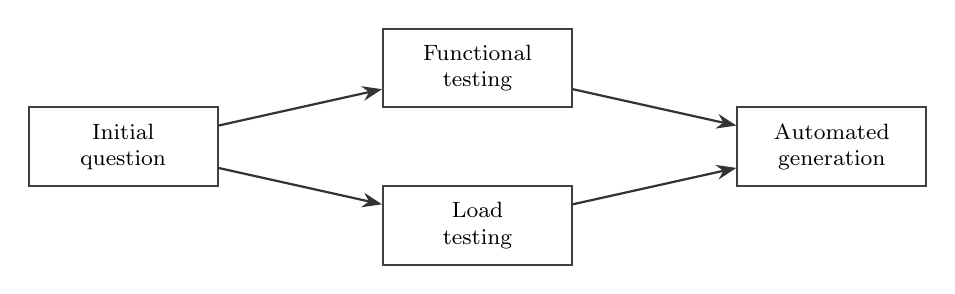
\begin{tikzpicture}[>={Stealth[length=2.5mm]}]
\node[ablock]   (q) at (-5.5,0)    {Initial\\question};
\node[ablock]   (f) at (-1.0, 1.0) {Functional\\testing};
\node[ablock]   (l) at (-1.0,-1.0) {Load\\testing};
\node[ablock]   (a) at ( 3.5,0)    {Automated\\generation};

\draw[aflow] (q) -- node[asig, above, sloped] {} (f);
\draw[aflow] (q) -- node[asig, below, sloped] {} (l);
\draw[aflow] (f) -- (a);
\draw[aflow] (l) -- (a);
\end{tikzpicture}
\end{center}

\vspace{0.8em}
\begin{center}
\textbf{Under what conditions can functional and load testing be \emph{systematically synthesised}\\
from declarative artefacts, rather than authored procedurally per service?}
\end{center}

\end{frame}

% --------- 3. What we needed -------------------------------------------
\begin{frame}{The artefact at the centre: the specification}

\begin{center}
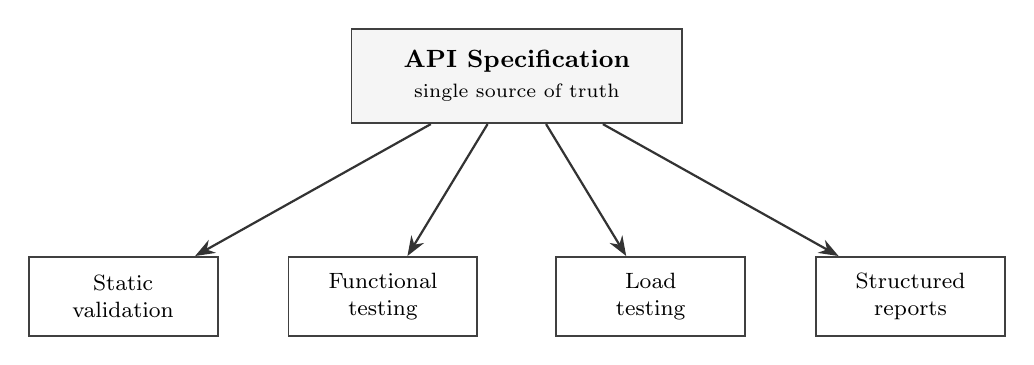
\begin{tikzpicture}[>={Stealth[length=2.5mm]}]
\node[asubject, minimum width=4.2cm, minimum height=1.2cm,
      font=\small\bfseries] (spec) at (0,1.8) {API Specification\\\scriptsize\textnormal{single source of truth}};

\node[ablock] (v) at (-5,  -1) {Static\\validation};
\node[ablock] (f) at (-1.7,-1) {Functional\\testing};
\node[ablock] (l) at ( 1.7,-1) {Load\\testing};
\node[ablock] (r) at ( 5,  -1) {Structured\\reports};

\draw[aflow] (spec) -- (v);
\draw[aflow] (spec) -- (f);
\draw[aflow] (spec) -- (l);
\draw[aflow] (spec) -- (r);
\end{tikzpicture}
\end{center}

\vspace{0.8em}
\begin{center}
This thesis formalises the resulting paradigm as \alert{\textbf{Specification-Driven Testing (SDT)}}.\\[0.4em]
\footnotesize Each derivation is realised as an orthogonal, composable operation in a unified CLI implementation.
\end{center}

\end{frame}

% --------- 3b. Research questions --------------------------------------
\begin{frame}{Research questions}

\footnotesize
\textbf{RQ1} --- Can automated API quality assurance be operationalised \emph{without dedicated human testers gating the promotion path}, while preserving deterministic and reproducible outcomes?

\vspace{0.6em}
\textbf{RQ2} --- To what extent can validation rules, executable test cases, and promotion gates be \emph{mechanically derived} from a single OpenAPI specification?

\vspace{0.6em}
\textbf{RQ3} --- How effectively does specification-driven QA compose with cloud-native, GitOps-governed delivery pipelines under continuous reconciliation?

\vspace{0.6em}
\textbf{RQ4} --- Can quality-gated delivery pipelines themselves be expressed as \emph{Kubernetes-native, ontologically structured specifications} --- discoverable, introspectable, and machine-actionable by both operators and autonomous agents?

\vspace{0.8em}
\begin{center}
\alert{Four questions, one unified specification-driven answer.}
\end{center}

\end{frame}

% --------- 3c. Spec drift: the silent problem -------------------------
\begin{frame}{The silent problem: specification--implementation divergence}

\vspace{-0.4em}
\begin{center}
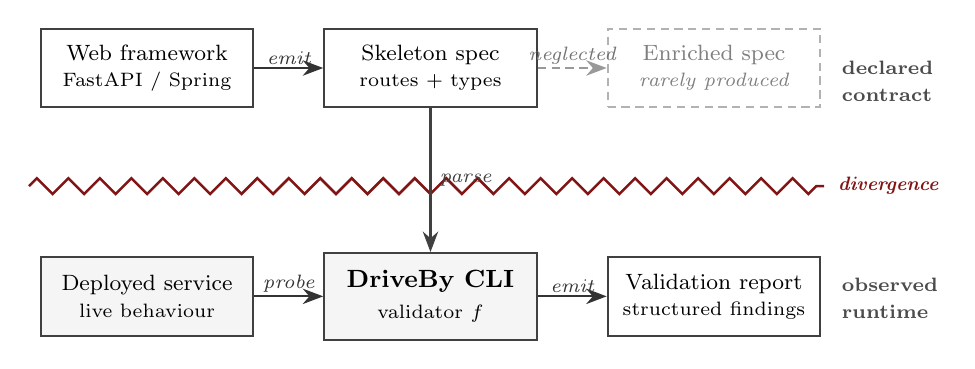
\begin{tikzpicture}[>={Stealth[length=2.6mm]}, font=\small]

% =====================================================================
% Top register: the declared contract (what tooling sees)
% =====================================================================
\node[ablock, minimum width=2.7cm] (fw)
  at (-3.6, 2.1) {Web framework\\\scriptsize FastAPI / Spring};
\node[ablock, minimum width=2.7cm] (skel)
  at ( 0.0, 2.1) {Skeleton spec\\\scriptsize routes $+$ types};
\node[ablock, minimum width=2.7cm, draw=black!30, text=black!50,
      densely dashed]
  (enr)  at ( 3.6, 2.1) {Enriched spec\\\scriptsize \itshape rarely produced};

\node[anchor=west, font=\scriptsize\bfseries, text=black!70]
  at (5.1, 2.1) {declared};
\node[anchor=west, font=\scriptsize\bfseries, text=black!70]
  at (5.1, 1.75) {contract};

\draw[aflow] (fw) -- node[asig, above] {emit} (skel);
\draw[->, line width=0.8pt, black!40, densely dashed]
  (skel) -- node[asig, above, text=black!55, font=\scriptsize\itshape] {neglected} (enr);

% =====================================================================
% Divergence band (red zigzag separating the two registers)
% =====================================================================
\draw[decorate, decoration={zigzag, segment length=4mm, amplitude=1mm},
      line width=0.9pt, sdtred!70!black]
  (-5.1, 0.6) -- (5.0, 0.6);
\node[anchor=west, font=\scriptsize\bfseries\itshape, text=sdtred!70!black,
      fill=white, inner sep=2pt]
  at (5.1, 0.6) {divergence};

% =====================================================================
% Bottom register: observed runtime
% =====================================================================
\node[ablock, minimum width=2.7cm, fill=black!4]
  (live) at (-3.6, -0.8) {Deployed service\\\scriptsize live behaviour};
\node[asubject, minimum width=2.7cm, minimum height=1.1cm,
      font=\small\bfseries]
  (cli)  at ( 0.0, -0.8) {DriveBy CLI\\\scriptsize\textnormal{validator $f$}};
\node[ablock, minimum width=2.7cm]
  (rep)  at ( 3.6, -0.8) {Validation report\\\scriptsize structured findings};

\node[anchor=west, font=\scriptsize\bfseries, text=black!70]
  at (5.1, -0.65) {observed};
\node[anchor=west, font=\scriptsize\bfseries, text=black!70]
  at (5.1, -1.00) {runtime};

\draw[aflow] (live) -- node[asig, above] {probe} (cli);
\draw[aflow] (cli)  -- node[asig, above] {emit} (rep);

% =====================================================================
% Cross-register validation: spec --> CLI
% =====================================================================
\draw[->, line width=0.8pt, black!75]
  (skel.south) -- node[asig, right=2pt, pos=0.5] {parse} (cli.north);

\end{tikzpicture}
\end{center}

\vspace{-0.4em}
\scriptsize
\begin{itemize}\setlength\itemsep{0.15em}
\item Web frameworks emit a \emph{structural skeleton}; \alert{none preserves
  specification--implementation parity over time}.
\item No framework \alert{enriches the contract} with the semantic descriptors
  --- operation summaries, error semantics, examples, security schemes ---
  that render it consumable by humans, tooling, and autonomous agents.
\item DriveBy treats the running service as ground truth: it probes the
  \emph{live contract}, compares it against the declared specification,
  and surfaces divergence as structured, actionable findings.
\end{itemize}

\end{frame}

% --------- 4. The DriveBy CLI ------------------------------------------
\begin{frame}{DriveBy: the reference implementation}

\begin{center}
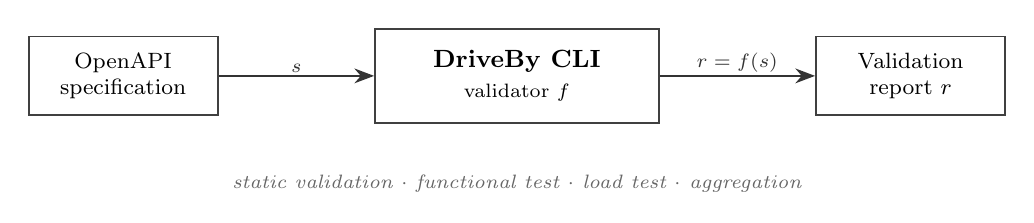
\begin{tikzpicture}[>={Stealth[length=2.5mm]}]
\node[ablock] (in)  at (-5,0) {OpenAPI\\specification};
\node[ablock, minimum width=3.6cm, minimum height=1.2cm,
      font=\small\bfseries] (cli) at (0,0) {DriveBy CLI\\\scriptsize\textnormal{validator $f$}};
\node[ablock] (out) at ( 5,0) {Validation\\report $r$};

\draw[aflow] (in)  -- node[asig, above] {$s$} (cli);
\draw[aflow] (cli) -- node[asig, above] {$r = f(s)$} (out);

\node[asig, below=0.6cm of cli, text=black!60]
  {static validation $\cdot$ functional test $\cdot$ load test $\cdot$ aggregation};
\end{tikzpicture}
\end{center}

\vspace{0.8em}
\footnotesize
\begin{itemize}\setlength\itemsep{0.3em}
\item Single Go binary; deterministic by construction: $f(s) = r$ for every spec $s$.
\item Structured JSON output: simultaneously human-interpretable and machine-actionable.
\item Each validation principle is an atomic, side-effect-free function over $s$ ---
  composable into higher-order validation policies.
\end{itemize}

\end{frame}

% --------- 5. Reality in industry today --------------------------------
\begin{frame}{Industrial practice vs.\ the SDT proposition}

\begin{columns}[T,onlytextwidth]

\column{0.48\textwidth}
\textbf{\textcolor{sdtred}{Industrial practice}}\\[0.4em]
\footnotesize
\begin{itemize}\setlength\itemsep{0.25em}
\item QA fragmented across siloed actors with no shared protocol.
\item Verification reduced to discretionary, ad-hoc sign-offs.
\item Expert capacity consumed by repetitive procedure --- diverted from
  process improvement.
\end{itemize}

\column{0.48\textwidth}
\textbf{\textcolor{sdtgreen}{SDT contribution}}\\[0.4em]
\footnotesize
\begin{itemize}\setlength\itemsep{0.25em}
\item Unified framework with structured, machine-actionable artefacts.
\item Each verification step is a deterministic, executable operation.
\item Human effort redirected from procedure to
  \emph{methodological improvement}.
\item QA promoted to \alert{first-class system component}.
\end{itemize}

\end{columns}

\vspace{0.8em}
\begin{center}
\alert{The bottleneck is not the testing --- it is the manual
choreography that surrounds it.}
\end{center}

\end{frame}

% --------- 6. Cloud-native deployment: declarative composition --------
\begin{frame}{Cloud-native delivery as a Kubernetes-native specification}

\begin{center}
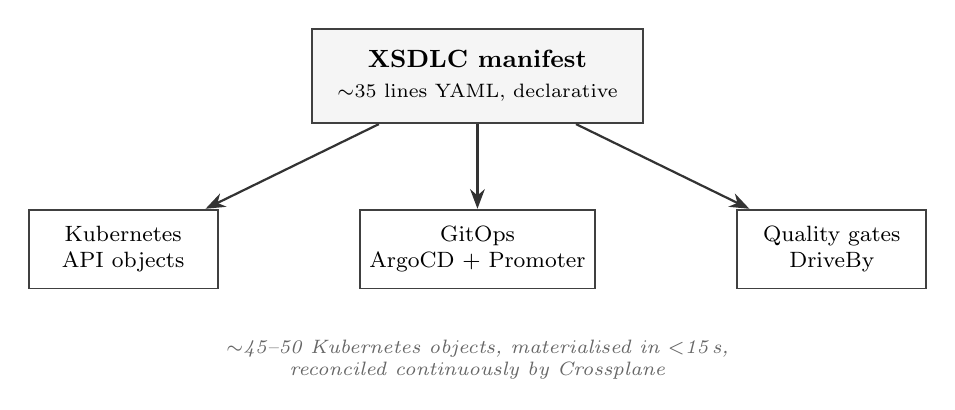
\begin{tikzpicture}[>={Stealth[length=2.5mm]}]
\node[asubject, minimum width=4.2cm, minimum height=1.2cm,
      font=\small\bfseries] (cr) at (0,2.2) {XSDLC manifest\\\scriptsize\textnormal{$\sim$35 lines YAML, declarative}};

\node[ablock] (k8s)    at (-4.5, 0) {Kubernetes\\API objects};
\node[ablock] (gitops) at ( 0,   0) {GitOps\\ArgoCD + Promoter};
\node[ablock] (gates)  at ( 4.5, 0) {Quality gates\\DriveBy};

\draw[aflow] (cr) -- (k8s);
\draw[aflow] (cr) -- (gitops);
\draw[aflow] (cr) -- (gates);

\node[asig, text=black!60, align=center] at (0,-1.4)
  {$\sim$45--50 Kubernetes objects, materialised in $<$15\,s,\\
   reconciled continuously by Crossplane};
\end{tikzpicture}
\end{center}

\vspace{0.2em}
\begin{center}
\footnotesize Identical declarative idiom to the API specification itself ---
\alert{the delivery pipeline is itself a structurally typed,
machine-discoverable specification.}
\end{center}

\end{frame}

% --------- 7. Consumers of the system ---------------------------------
\begin{frame}{System consumers}

\begin{center}
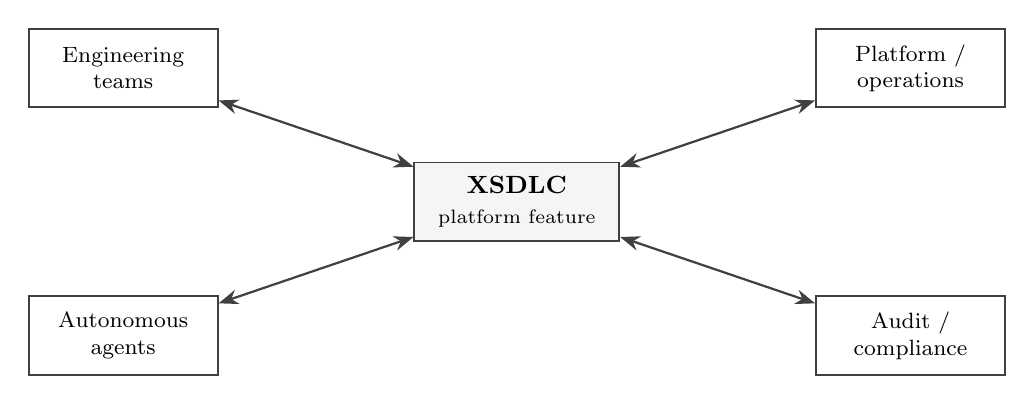
\begin{tikzpicture}[>={Stealth[length=2.5mm]}]
\node[asubject, minimum width=2.6cm, minimum height=1.0cm,
      font=\small\bfseries] (sdt) at (0,0) {XSDLC\\\scriptsize\textnormal{platform feature}};

\node[ablock] (eng)   at (-5.0, 1.7) {Engineering\\teams};
\node[ablock] (ops)   at ( 5.0, 1.7) {Platform /\\operations};
\node[ablock] (agent) at (-5.0,-1.7) {Autonomous\\agents};
\node[ablock] (audit) at ( 5.0,-1.7) {Audit /\\compliance};

\draw[<->, line width=0.8pt, black!75] (sdt) -- (eng);
\draw[<->, line width=0.8pt, black!75] (sdt) -- (ops);
\draw[<->, line width=0.8pt, black!75] (sdt) -- (agent);
\draw[<->, line width=0.8pt, black!75] (sdt) -- (audit);
\end{tikzpicture}
\end{center}

\vspace{0.2em}
\scriptsize
\begin{itemize}\setlength\itemsep{0.15em}
\item \textbf{Engineers} --- declare desired state; XSDLC reifies it.
\item \textbf{Operations} --- interact via standard Kubernetes-native primitives; zero proprietary surface area.
\item \textbf{Autonomous agents} --- consume structured findings as a closed-form, machine-actionable feedback signal.
\item \textbf{Audit \& compliance} --- inherit reproducible, machine-verifiable evidence with intrinsic provenance.
\end{itemize}

\end{frame}

% --------- 8. Control loop: academic block diagram --------------------
\begin{frame}{Closed-loop quality control: block diagram}

\vspace{-0.3em}
\begin{center}
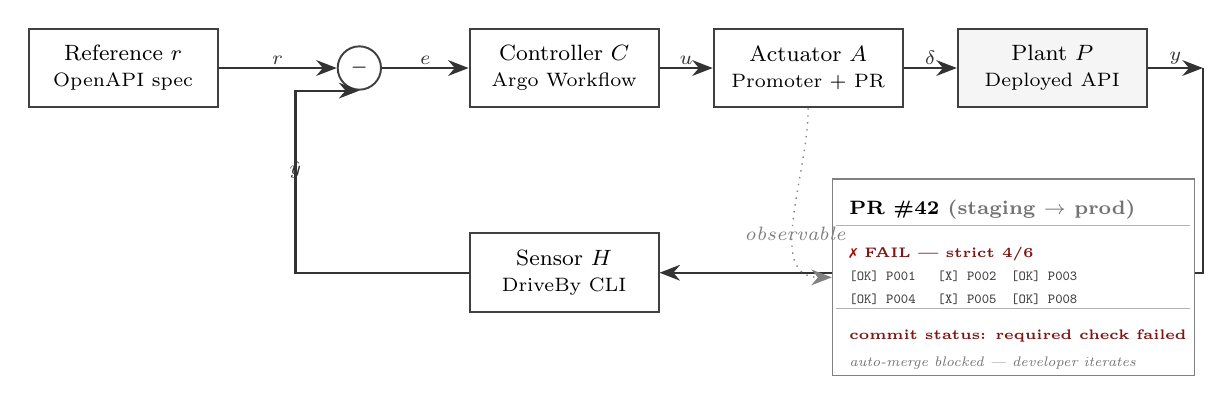
\begin{tikzpicture}[
    >={Stealth[length=2.6mm,width=2mm]},
    font=\small,
    block/.style={rectangle, draw=black!75, fill=white,
                  minimum width=2.4cm, minimum height=1.0cm,
                  align=center, font=\footnotesize, line width=0.7pt},
    plant/.style={rectangle, draw=black!75, fill=black!4,
                  minimum width=2.4cm, minimum height=1.0cm,
                  align=center, font=\footnotesize, line width=0.7pt},
    sumnode/.style={circle, draw=black!75, fill=white,
                    minimum size=0.55cm, inner sep=0pt,
                    font=\scriptsize, line width=0.7pt},
    sig/.style={font=\scriptsize\itshape, inner sep=1pt},
    flow/.style={->, line width=0.8pt, black!80}]

% --- Forward path: r --> sum --> C --> A --> P --> y -------------------
\node[block] (ref)  at (0,    0) {Reference $r$\\\scriptsize OpenAPI spec};
\node[sumnode] (sum) at (3.0,  0) {};
\node[sig] at (3.0,0) {$-$};
\node[block] (ctrl) at (5.6,  0) {Controller $C$\\\scriptsize Argo Workflow};
\node[block] (act)  at (8.7,  0) {Actuator $A$\\\scriptsize Promoter + PR};
\node[plant] (plant) at (11.8, 0) {Plant $P$\\\scriptsize Deployed API};

\draw[flow] (ref)  -- node[sig, above] {$r$} (sum);
\draw[flow] (sum)  -- node[sig, above] {$e$} (ctrl);
\draw[flow] (ctrl) -- node[sig, above] {$u$} (act);
\draw[flow] (act)  -- node[sig, above] {$\delta$} (plant);

% Output y emerging from plant
\draw[flow] (plant.east) -- ++(0.7,0)
  node[sig, above, pos=0.5] {$y$}
  coordinate (yout);

% --- Feedback path: y -> sensor -> measurement -> sum ------------------
\node[block] (sensor) at (5.6, -2.6) {Sensor $H$\\\scriptsize DriveBy CLI};

\draw[flow] (yout) |- (sensor.east);
\draw[flow] (sensor.west) -- ++(-2.2,0) |- node[sig, above, pos=0.25] {$\hat{y}$} (sum.south);

% --- Visual zoom-in: PR commit-status snapshot (right side, below y) ---
\node[draw=black!50, line width=0.5pt, fill=white,
      minimum width=4.6cm, minimum height=2.5cm,
      anchor=north west] (pr) at (9.0, -1.4) {};

\node[anchor=north west, font=\scriptsize\bfseries]
  at (9.1, -1.55) {PR \#42 \textcolor{black!55}{(staging $\to$ prod)}};
\draw[black!30] (9.05, -2.0) -- (13.55, -2.0);

\node[anchor=north west, font=\tiny\bfseries, text=sdtred!70!black]
  at (9.1, -2.15) {\xmark\ FAIL --- strict 4/6};
\node[anchor=north west, font=\tiny\ttfamily, text=black!75]
  at (9.1, -2.45) {[OK] P001\ \ \ [X] P002\ \ [OK] P003};
\node[anchor=north west, font=\tiny\ttfamily, text=black!75]
  at (9.1, -2.75) {[OK] P004\ \ \ [X] P005\ \ [OK] P008};
\draw[black!30] (9.05, -3.05) -- (13.55, -3.05);
\node[anchor=north west, font=\tiny\bfseries, text=sdtred!70!black]
  at (9.1, -3.20) {commit status: required check failed};
\node[anchor=north west, font=\tiny\itshape, text=black!55]
  at (9.1, -3.55) {auto-merge blocked --- developer iterates};

% Dotted "this is what the actuator emits" arrow from A to PR
\draw[->, line width=0.5pt, black!50, dotted]
  (act.south) to[out=-90,in=180] node[sig, midway, below=2pt] {observable} (pr.west);

\end{tikzpicture}
\end{center}

\vspace{-0.2em}
\begin{center}
\footnotesize
$e(t) = r(t) - H\!\left(y(t)\right)$ \quad
with $r$ the declared OpenAPI specification,
$y$ the observed runtime behaviour, and $H$ the DriveBy validator.\\[0.15em]
The promotion gate is the actuator; deviation closes the loop continuously.
\end{center}

\end{frame}

% --------- 8b. Empirical evidence -------------------------------------
\begin{frame}{Empirical evidence: prevalence and remediability}

\begin{columns}[T,onlytextwidth]

\column{0.48\textwidth}
\textbf{\textcolor{sdtblue}{Systemic quality gap}}\\[0.4em]
\footnotesize
70 distinct providers from APIs.guru\\
(50 OpenAPI 3.x + 20 Swagger 2.0)\\[0.4em]
\alert{84\% score $\leq 1/6$ under the strict policy.}\\[0.4em]
\textcolor{gray}{No specimen in the sample satisfies more than 2 of the 6 evaluated principles --- a systemic, cross-vendor deficiency.}

\column{0.48\textwidth}
\textbf{\textcolor{sdtgreen}{Agent-actionable feedback}}\\[0.4em]
\footnotesize
Swagger Petstore baseline: \textbf{1/6}.\\
After a single iteration of an AI coding agent receiving \emph{only} the DriveBy JSON report:\\[0.4em]
\alert{4/6 ($+$300\%).}\\[0.4em]
\textcolor{gray}{No remediation prompt. No exemplar. The structured findings alone sufficed.}

\end{columns}

\vspace{1em}
\begin{center}
\footnotesize SDT's structured output is sufficient feedback for
\emph{both} human practitioners \emph{and} autonomous agents ---
empirically validating its machine-actionable semantics.
\end{center}

\end{frame}

% --------- 9. Empirical contribution: the payoff ----------------------
\begin{frame}{Quantified contribution: from days of manual toil to a self-reconciling system}

\begin{columns}[T,onlytextwidth]

\column{0.48\textwidth}
\textbf{\textcolor{sdtred}{Conventional practice}}\\[0.4em]
\footnotesize
\begin{itemize}\setlength\itemsep{0.25em}
\item Multi-day provisioning per service: quality gates, repositories, branches, identities, ingress routes --- each wired by hand.
\item Configuration drift discovered \emph{post-incident}, not pre-emptively.
\item QA reduced to a sequence of human sign-offs --- non-reproducible, non-auditable.
\end{itemize}

\column{0.48\textwidth}
\textbf{\textcolor{sdtgreen}{This thesis (SDT $+$ XSDLC)}}\\[0.4em]
\footnotesize
\begin{itemize}\setlength\itemsep{0.25em}
\item One declarative manifest; full pipeline materialised in $<$15\,s.
\item \alert{Drift detected \emph{and} reconciled} ---
  \textbf{11 of 12} injected drift scenarios converged automatically.
\item Every lifecycle event is \alert{auditable and discoverable} via the Kubernetes API --- machine-readable provenance for every change.
\item QA promoted from human procedure to a \emph{first-class system component}.
\end{itemize}

\end{columns}

\vspace{0.8em}
\begin{center}
\alert{What previously required days of expert manual effort is now provisioned, governed,
and \emph{self-reconciled} by the platform --- with full observability and audit traceability.}
\end{center}

\end{frame}

% --------- 10. Closing -------------------------------------------------
\begin{frame}{Contributions}

\begin{center}
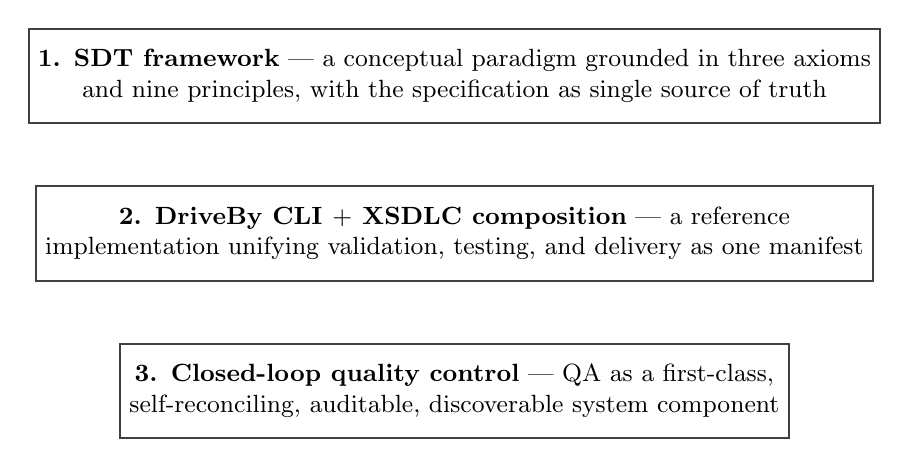
\begin{tikzpicture}
\node[ablock, minimum width=8.5cm, minimum height=1.2cm,
      font=\small] (a) at (0, 2.0)
  {\textbf{1. SDT framework}\ ---\ a conceptual paradigm grounded in three axioms\\
   and nine principles, with the specification as single source of truth};
\node[ablock, minimum width=8.5cm, minimum height=1.2cm,
      font=\small] (b) at (0, 0.0)
  {\textbf{2. DriveBy CLI $+$ XSDLC composition}\ ---\ a reference\\
   implementation unifying validation, testing, and delivery as one manifest};
\node[ablock, minimum width=8.5cm, minimum height=1.2cm,
      font=\small] (c) at (0,-2.0)
  {\textbf{3. Closed-loop quality control}\ ---\ QA as a first-class,\\
   self-reconciling, auditable, discoverable system component};
\end{tikzpicture}
\end{center}

\vspace{1em}
\begin{center}
\Large\textbf{Thank you.}\\[0.4em]
\normalsize Questions?
\end{center}

\end{frame}

\end{document}
